\subsection{Проектирование и разработка серверной части программного средства}
\label{sec:design:server}

\subsubsection{} Этапы разработки программного средства
\label{sec:design:server:overview}

Архитектурный стиль разделения функциональности программной системы на уровни поднимает сразу несколько проблем.
Их решение в типичном случае заключается в выполнении следующих этапов~\cite{application_architecture_guide}:

\begin{enumerate}
	\item определение стратегии разбиения на уровни;
	\item определение уровней;
	\item распределение функциональности по уровням и компонентам;
	\item уточнение количества уровней: при необходимости некоторые из них объединяются;
	\item установление правил взаимодействия уровней;
	\item идентификация функциональности, которая используется на всех\linebreak уровнях (cross cutting concerns);
	\item определение интерфейсов уровней;
	\item выбор стратегии развертывания;
	\item выбор конкретных протоколов взаимодействия.
\end{enumerate}

К данному этапу разработки дипломного проекта выполнены шаги с \ref{sec:design:server:overview}а по
\ref{sec:design:server:overview}д. Шаг \ref{sec:design:server:overview}е вследствие использования различных
программных средств, применяемых на уровнях, будет выполняться позднее -- на соответствующих уровнях.

Таким образом, следующий этап -- это определение интерфейсов уровней. СУБД имеет заранее определенный интерфейс,
установленный ее разработчиком. Предполагается, что из остальных двух частей программной системы инициатором любых
действий будет являться клиентская. Следовательно, единственный межуровневый интерфейс, который следует определить --
это интерфейс серверной части.

Веб-приложения, в стиле которых планируется создание клиентской части, обычно запускаются большим числом
пользователей. Таким образом очевидна автономность и независимость частей проектируемой программной системы.
Исходя из этих соображений, целесообразным является применение сервис-ориентированного архитектурного стиля.

\subsubsection{} Программный интерфейс серверной части
\label{sec:design:server:interface}

Предварительным условием для проектирования серверной части приложения является определение его интерфейса в
высокоуровневых терминах предметной области. Таким образом, далее приведены методы его API, которые основаны на
функциональных требованиях, определенных\linebreakв подразделе~\ref{sec:domain:specification}:

\begin{itemize}
	\item метод регистрации пользователя системы, принимающий адрес электронной почты, пароль, повторный пароль;
	\item метод смены пароля, также принимающий старый пароль, новый пароль, повторный новый пароль;
	\item метод аутентификации, принимающий пароль и адрес электронной почты;
	\item метод восстановления пароля, принимающий адрес электронной почты;
	\item метод приглашения нового пользователя, принимающий адрес электронной почты;
	\item метод принятия приглашения пользователя, принимающий пароль, повторный пароль;
	\item метод, возвращающий список пользователей;
	\item метод, возвращающий список копий профилей;
	\item метод создания копии профиля;
	\item метод, возвращающий копию профиля для редактирования;
	\item метод просмотра копии профлия;
	\item метод обновления данных копии профиля;
	\item метод удаления копии профиля;
	\item метод, возвращающий список статусов профилей;
	\item метод, возвращающий список навыков;
	\item метод, возвращающий список ролей системы;
	\item метод, возвращающий список прав для ролей;
	\item метод обновления прав;
	\item метод создания департамента;
	\item метод просмотра департамента;
	\item метод обновления департамента;
	\item метод удаления департамента;
	\item метод создания вопроса;
	\item метод просмотра вопроса;
	\item метод обновения вопроса;
	\item метод удаления вопроса;
	\item метод, возвращающий список проектов;
	\item метод создания нового проекта;
	\item метод, возвращающий проект для редактирования;
	\item метод просмотра проекта;
	\item метод обновения проекта;
	\item метод удаления проекта;
	\item метод, возвращающий список позиций;
	\item метод создания новой позиции;
	\item метод, возвращающий позицию для редактирования;
	\item метод просмотра позиции;
	\item метод обновения позиции;
	\item метод удаления позиции;
	\item метод, возвращающий список категорий;
	\item метод, возвращающий категорию для редактирования;
	\item метод просмотра категории;
	\item метод обновления категории;
	\item метод удаления категории;
	\item метод назначения менеджеров на департаменты;
	\item метод, возвращающий менеджеров департаментов;
	\item метод, возвращающий списки прав;
	\item метод, возвращающий информацию о текущем пользователей;
	\item метод просмотра информации о пользователе;
	\item метод, возвращающий список технологий;
	\item метод, возвращающий список департаментов;
	\item метод, возвращающий список вопросов для позиции;
	\item метод, возвращающий список позиций;
	\item метод, возвращающий список проектов;
	\item метод, возвращающий список вопросов;
	\item метод создания профиля пользователя;
	\item метод просмотра профиля пользователя;
	\item метод обновения профиля пользователя;
	\item метод отправки профиля на модерацию;
	\item метод генерации резюме;
	\item метод обновления фотографии профиля.
\end{itemize}

На рисунке~\ref{fig:design:server:interface:server_algorithm} приведена схема алгоритма обработки запросов
перечисленных методов программного интерфейса серверной частью приложения. Далее приведены архитектурные решения,
которые были применены при реализации данной части программной системы. 

Поскольку в ПС проектируется реализация сложных независимых систем ролей и пользовательских функций, которые находят
своё отражение в серверной части приложения, то встаёт вопрос об их сопряжении. А поскольку данное сопряжение
вследствие особенностей предметной области является достаточно нетривиальным: часть функций уникальна для некоторых
ролей, часть разделяется ими всеми. Поэтому целесообразным является разбиение их на следующие группы:

\begin{enumerate}
	\item функции, доступные без аутентификации;
	\item функции, доступные для всех аутентифицированных пользователей;
	\item функции менеджеров;
	\item функции администраторов.
\end{enumerate}

\begin{sidewaysfigure}
  \centering
    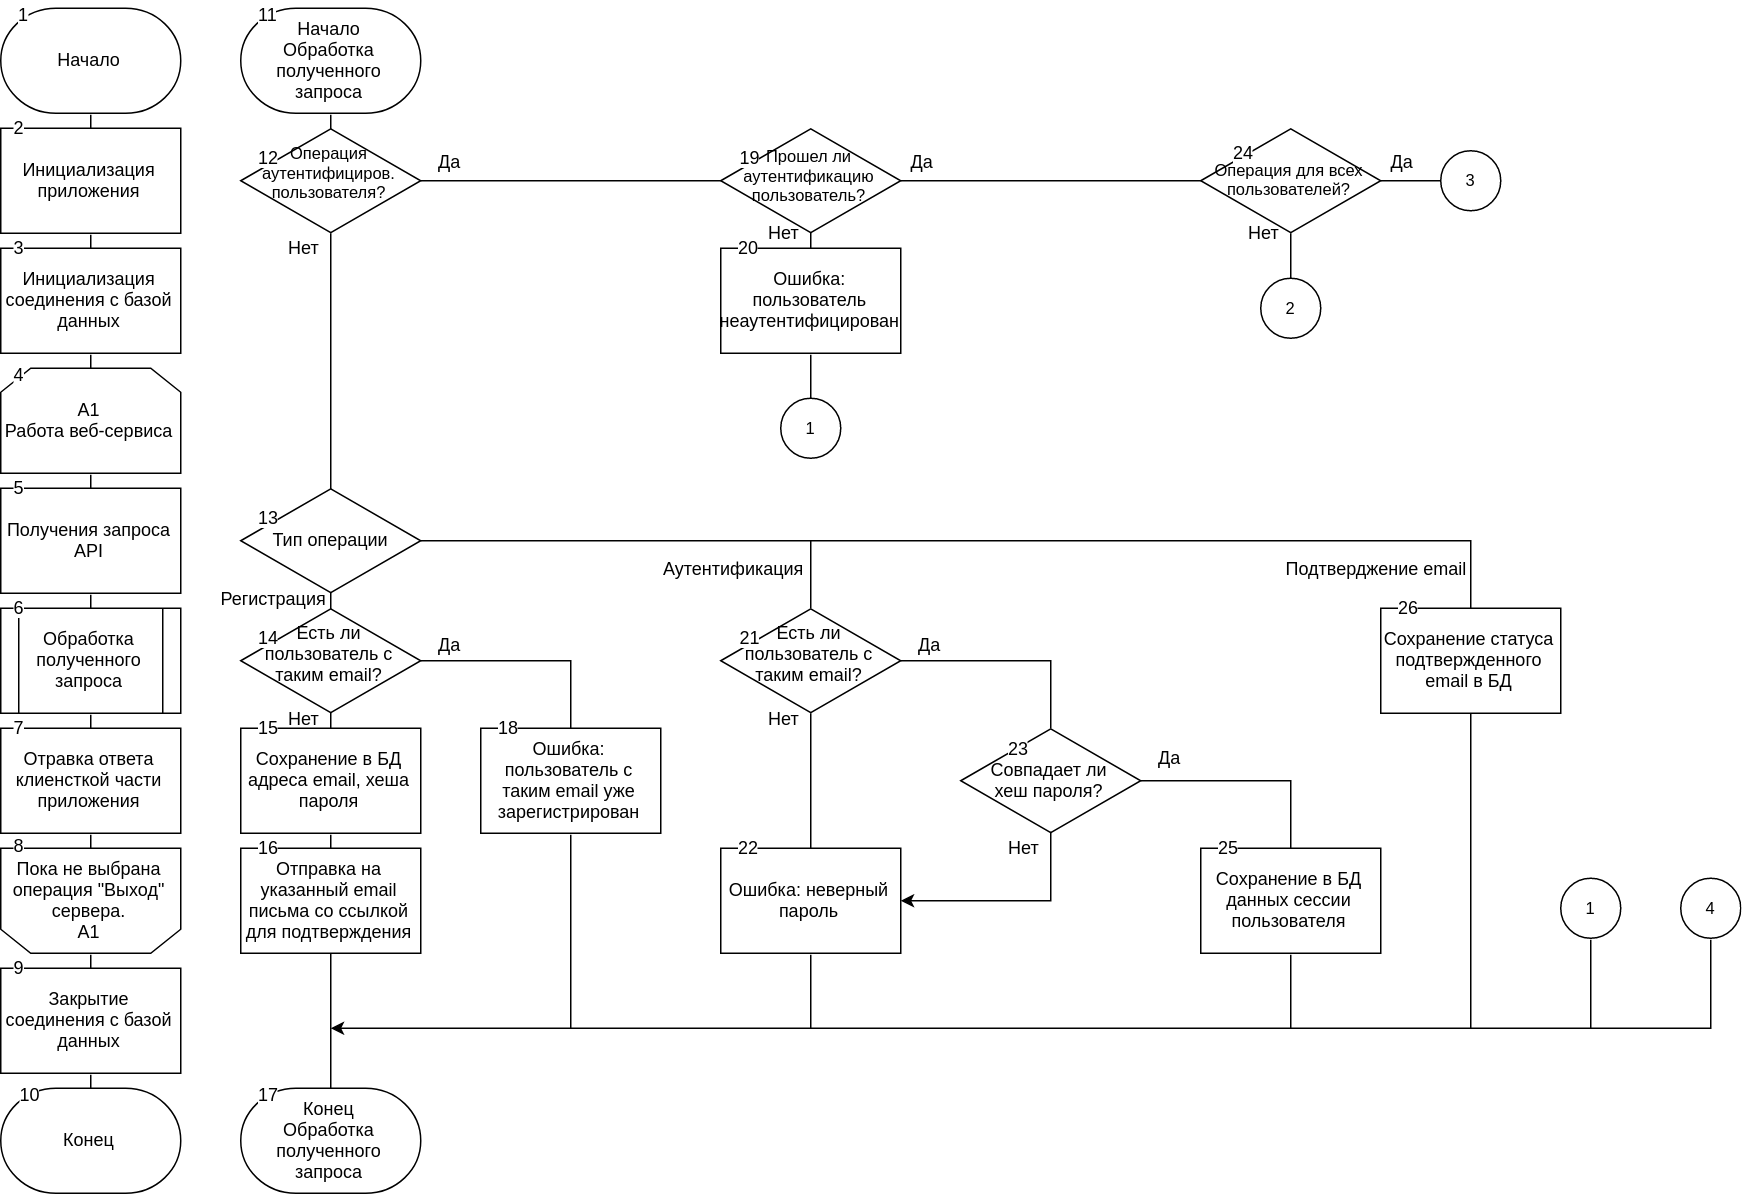
\includegraphics[scale=0.37]{server-algorithm-1.png}
    \caption{Схема программы серверной части программного средства}
    \label{fig:design:server:interface:server_algorithm}
\end{sidewaysfigure}

\begin{sidewaysfigure}
  \ContinuedFloat
  \centering
    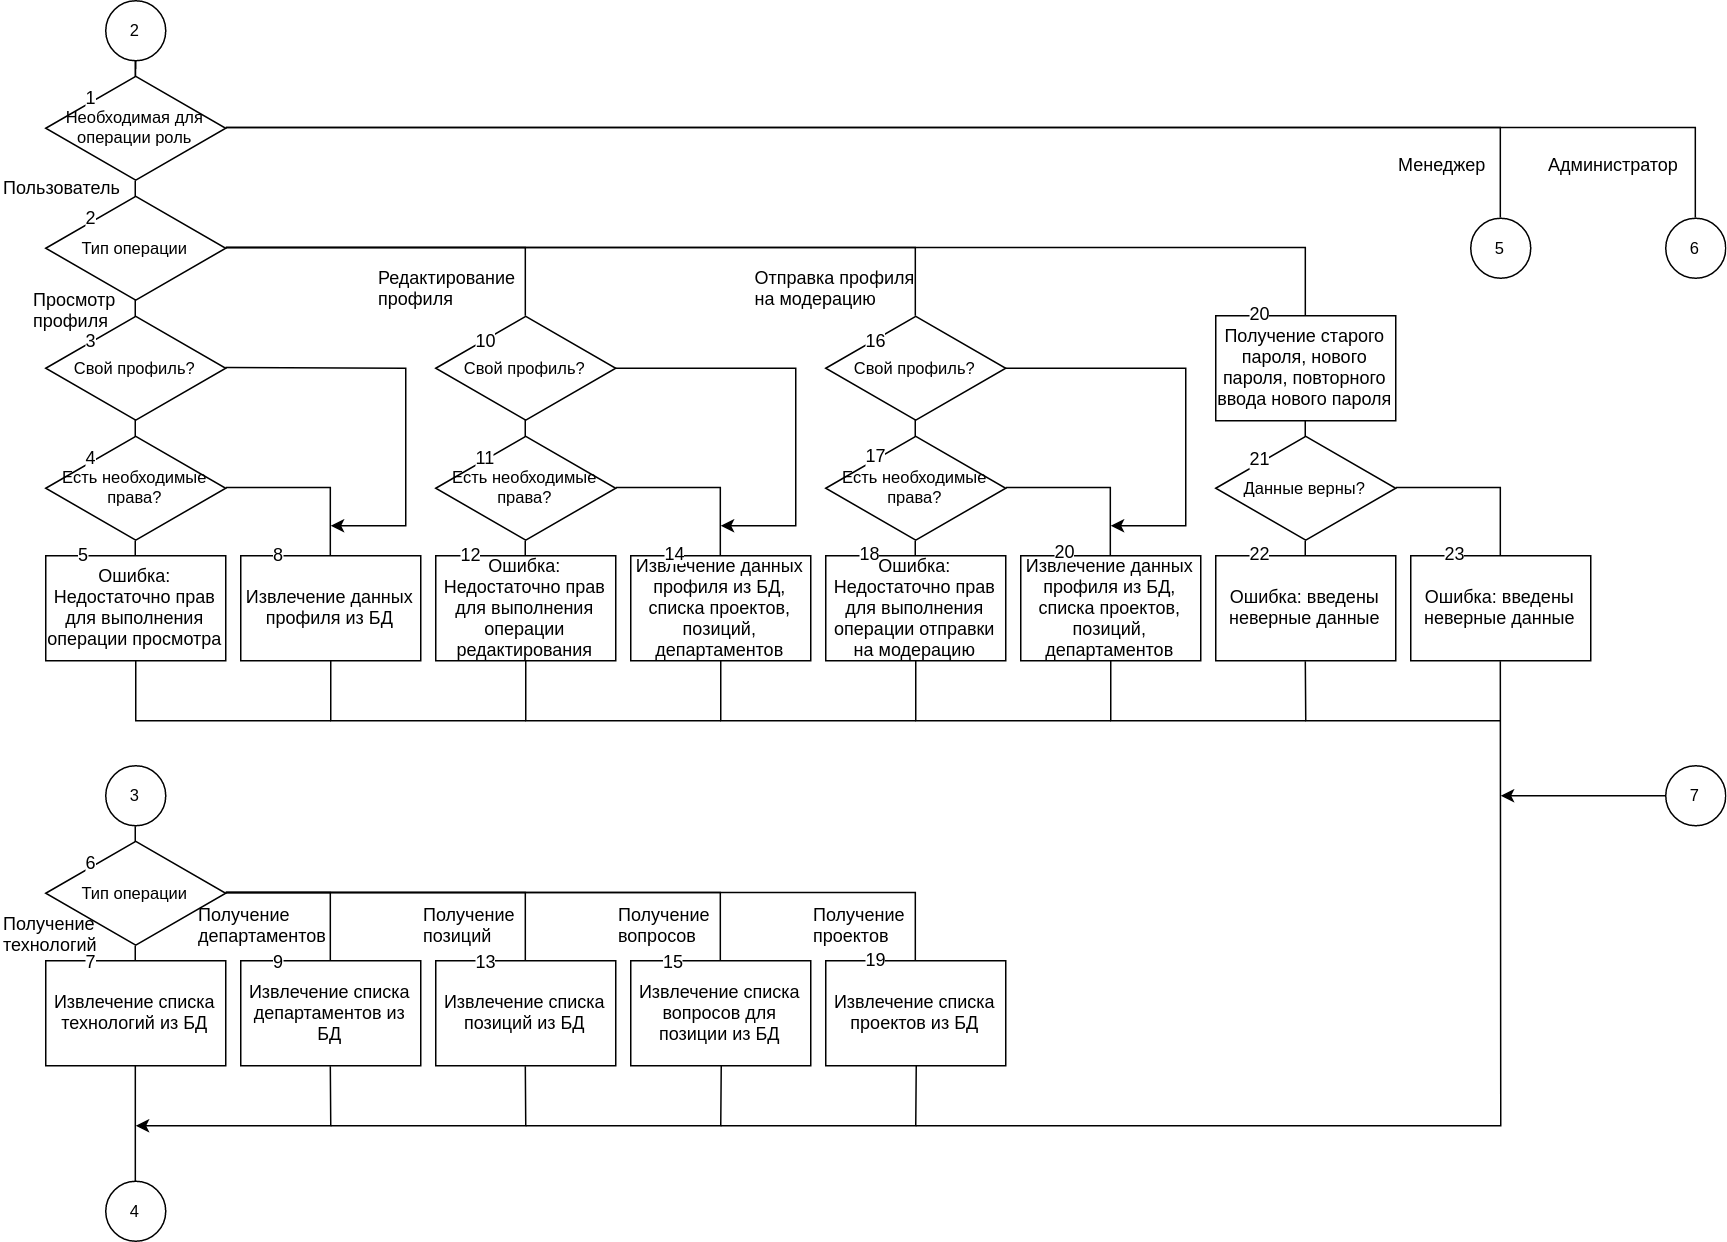
\includegraphics[scale=0.37]{server-algorithm-2.png}
    \caption{Схема программы серверной части программного средства (продолжение)}
\end{sidewaysfigure}
  
\begin{sidewaysfigure}
  \ContinuedFloat
  \centering
    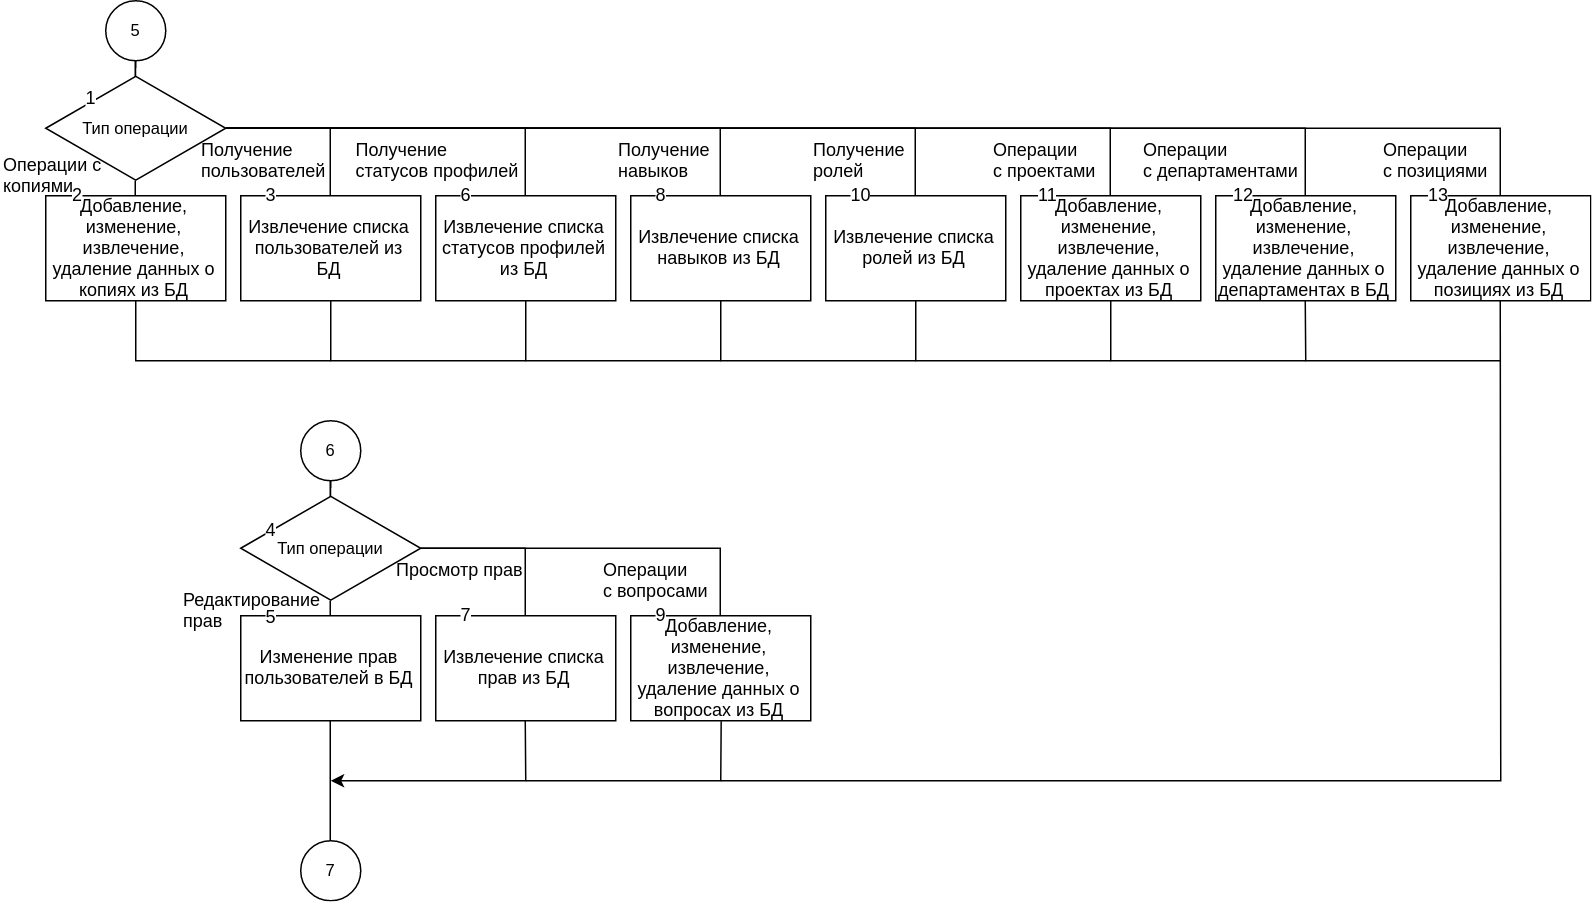
\includegraphics[scale=0.45]{server-algorithm-3.png}
    \caption{Схема программы серверной части программного средства (окончание)}
\end{sidewaysfigure}

Серверная проверка аутентификации пользователей будет осуществляться с помощью технологии создания и проверки
специального токена.

Большое количество блоков, в которых осуществляется доступ к БД, подтверждает назначение всей серверной части
приложения: прослойка между клиентским веб-приложением и базой данных с добавлением проверок аутентификации и авторизации.

Реализовав перечисленные методы API, можно будет достигнуть очень важной цели: внутренняя бизнес-логика, логика доступа
к данным и сами данные будут надежно защищены.

\subsubsection{} Выбор протоколов коммуникации
\label{sec:design:server:protocols}

В пункте~\ref{sec:design:server:overview} приведены этапы, в соответствии с которыми рекомендуется производить
проектирование программного системы~\cite{application_architecture_guide}. Этап \ref{sec:design:server:overview}з будет
рассмотрен позднее вследствие неоднородности и отсутствия схожести в применяющихся технологий между уровнями.
Таким образом, следующий актуальный этап -- \ref{sec:design:server:overview}и: выбор конкретных протоколов взаимодействия.

Можно выделить два основных стиля, которые (с необходимыми модификациями в каждом конкретном случае) применяются в
информационных системах, содержащих веб-сервисы~\cite{application_architecture_guide}: REST (Representational State
Transfer -- протокол передачи состояния представления) и SOAP (Simple Object Access Protocol -- простой протокол
доступа к объектам). Технически REST является архитектурным шаблоном проектирования, построенным на основе
использования простых глаголов (называемых запросами или методами). На практике данный архитектурный стиль применяется
в связке с протоколом прикладного уровня модели OSI HTTP. SOAP же является XML-ориентированным протоколом, причем
стандарт не специфицирует применяемые протоколы передачи данных.

Основное отличие между данными протоколами состоит в способе манипулирования состоянием. SOAP предусматривает
осуществление переходов между различными состояниями с помощью взаимодействия с единственной конечной точкой ввода
информации, через которую предоставляется доступ к функциональности сервиса. Протокол REST предполагает использование
ограниченного набора операций, которые могут применяться к ресурсам, адресуемым с помощью уникальных адресов URI. 

Данный протокол в большей степени соответствует распределенной архитектуре клиент-серверных приложений, поскольку
серверная часть публично доступна для множества заведомо неизвестных клиентских приложений. REST обладает свойством
отсутствия состояния, что означает, что каждый запрос должен содержать в себе достаточный набор данных для его
осуществления. Кроме того, данный протокол не запрещает использование различных форматов передачи данных,
например, JSON, что оказывается огромным преимуществом перед SOAP вследствие планируемого использования в клиентской
части языка Javascript, который нативно поддерживает данный формат.

\subsubsection{} Настройка окружения
\label{sec:design:server:environment}

Перед установкой Rails необходимо проверить, чтобы в системе были установлены необходимые предварительные зависимости.
К ним относятся Ruby и PostgreSQL.

Для установки Rails используется команду gem install, представленная RubyGems:

\begin{flushleft}
  \qquad\qquad\qquad \$ gem install rails
\end{flushleft}

Rails поставляется с рядом скриптов, названных генераторами, разработанных для облегчения жизни разработчика, создавая
все, что необходимо для начала работы над определенной задачей. Одним из них является генератор нового приложения,
предоставляющий основу приложения Rails, таким образом, не нужно писать его самостоятельно.

Для использования этого генератора создания приложения, необходимо в терминале выполнить следующую команду:

\begin{flushleft}
  \qquad\qquad\qquad \$ rails new diploma
\end{flushleft}

Это создаст приложение на Rails с именем Diploma в директории\linebreak diploma и установит гемы, зависимости от которых
упомянуты в Gemfile при использовании bundle install.

Как и в большинстве языков программирования, в Ruby можно использовать широкий набор сторонних библиотек.
Большая часть из них реализована в форме гема. RubyGems -- менеджер пакетов Ruby, созданный для упрощения процесса
создания, распространения и установки библиотек.

В директории diploma имеется несколько автоматически сгенерированных файлов и папок, задающих структуру приложения
на Rails. Рассмотрим подробнее функциии каждой папки, которые создает Rails в новом приложении по умолчанию в
таблице~\ref{table:design:server:environment:structure}:

\begin{table}[!ht]
\caption{Назначение папок, используемых в проекте}
\label{table:design:server:environment:structure}
\centering
	\begin{tabular}{{ 
	|>{\centering}m{0.2\textwidth} | 
	 >{\raggedright\arraybackslash}m{0.74\textwidth}|}}

  	\hline
  	Название папки/файла & {\begin{center} Назначение \end{center}} \\

  	\hline
		app/ & Содержит контроллеры, модели, представления, хелперы, рассыльщики, каналы, задания и стили приложения.\\
		
		\hline
		bin/ & Содержит Rails скрипты которые стартуют приложение, также директория может содержать другие скрипты которые
		используются для настройки, обновления, деплоя или запуска.\\

		\hline
		config/	& Конфигурации маршрутов, базы данных приложения, и т.д.\\

		\hline
		config.ru &	Конфигурация Rack для серверов, основанных на Rack, используемых для запуска приложения. \\

		\hline
		db/ & Содержит текущую схему базы данных, а также миграции базы данных.\\

		\hline
		Gemfile\linebreak Gemfile.lock & Эти файлы позволяют указать, какие зависимости от гемов нужны для приложения на
		Rails. Эти файлы используются гемом Bundler.\\

		\hline
		lib/ & Внешние модули для приложения.\\

		\hline
		package.json & Этот файл позволяет указать, какие зависимости npm необходимы для приложения Rails.
		Этот файл используется Yarn. \\

		\hline
		public/ & Единственная папка, которая доступна извне как есть. Содержит статичные файлы и скомпилированные стили.\\

		\hline
		Rakefile & Этот файл находит и загружает задачи, которые могут быть запущены в командной строке. Определенная
		задача доступна во всех компонентах Rails. Вместо изменения Rakefile, можно добавить свои собственные задачи,
		добавив файлы в директорию lib/tasks приложения.\\

		\hline
		test/ & Юнит-тесты, и прочий аппарат тестирования\\
		
		\hline
		vendor/ & Место для кода сторонних разработчиков. В типичном приложении на Rails включает внешние гемы.\\

	\hline
	\end{tabular}
\end{table}

Для запуска веб-сервера на машине, необходимо запустить следующую команду из директории diploma:

\begin{flushleft}
  \qquad\qquad\qquad \$ bin/rails server
\end{flushleft}

Это запустит Puma, веб-сервер, распространяющийся с Rails по умолчанию. Чтобы увидеть приложение в действии, необходимо
открыть окно браузера и пройти по адресу http://localhost:3000.

\subsubsection{} Конструирование серверной части приложения
\label{sec:design:server:development}

Наконец, по завершению этапов проектирования и подготовки можно приступить к собственно созданию исходных кодов
приложения. Ключевые фрагменты кода, описание которых приведено в данном пункте, приведены в приложении A.

Чтобы добавить в Rails логику, нужно создать, как минимум, контроллер и представление.

Назначением контроллера является получение определенных запросов к приложению. Роутинг решает, какой контроллер получит
какие запросы. Часто имеется более одного маршрута к каждому контроллеру, и различные маршруты могут быть обработаны
различными экшнами. Назначением каждого экшна является сбор информации для предоставления ее на представление.

Назначением представления является отображение этой информации в удобочитаемом формате. Необходимо отметить важное различие,
что местом, в котором собирается информация, является контроллер, а не представление. Представление должна только лишь
отображать эту информацию. По умолчанию шаблоны представление пишутся на языке, названном eRuby (Embedded Ruby),
который конвертируется циклом запросов в Rails до отправки пользователю.

Для создания нового контроллера, нужно запустить генератор\linebreak"controller" и сказать, что необходим контроллер с именем
"Welcome" с экшном по имени "index", вот так:

\begin{flushleft}
  \qquad\qquad\qquad \$ bin/rails generate controller Welcome index
\end{flushleft}

Контроллер -- это просто класс, унаследованный от\linebreak ApplicationController. В этом классе необходімо определить методы,
которые станут экшнами для этого контроллера. Эти экшны будут выполнять операции CRUD с сущностями в системе.

Модели в Rails используют имя в единственном числе, а их соответствующая таблица в базе данных -- имя во множественном
числе. Rails предоставляет генератор для создания моделей, которым пользуются большинство разработчиков на Rails для
создания новых моделей. Для создания новой модели, необходимо эту команду в терминале:

\begin{flushleft}
  \qquad\qquad\qquad \$ bin/rails generate model Article title:string text:text
\end{flushleft}

С помощью этой команды Rails сообщают, что необходима модель\linebreak Article с атрибутом title строкового типа и атрибутом text
текстового типа. Эти атрибуты автоматически добавятся в таблицу articles и привяжутся к модели Article.

bin/rails generate model создал файл миграции базы данных в директории db/migrate. Миграции -- это класс Ruby,
разработанный для того, чтобы было просто создавать и модифицировать таблицы базы данных. Rails использует команды
rake для запуска миграций, и возможна отмена миграции после того, как она была применена к базе данных. Имя файла
миграции включает временную метку, чтобы быть уверенным, что они выполняются в той последовательности, в которой они
создавались.

чтобы запустить миграцию, необходимо использовать команду bin/rails:

\begin{flushleft}
  \qquad\qquad\qquad \$ bin/rails db:migrate
\end{flushleft}

Rails выполнит эту команду миграции и сообщит, что он создал таблицу Articles.

Роутер Rails распознает URL и направляет его в экшн контроллера или в приложение Rack. Он также может генерировать пути
и URL, избегая необходимость жестко прописывать строки в представлениях.

Маршруты для приложения или engine располагаются в файле\linebreak config/routes.rb и обычно выглядят так:

\begin{flushleft}
	\qquad\qquad\qquad Rails.application.routes.draw do\\
	\qquad\qquad\qquad\quad Rails.application.routes.draw do\\
	\qquad\qquad\qquad\quad\quad resources :products, only: [:index, :show]\\
	\qquad\qquad\qquad\quad end\\
	\qquad\qquad\qquad\quad resource :basket, only: [:show, :update, :destroy]\\
	\qquad\qquad\qquad\quad resolve("Basket") { route\_for(:basket) }\\
	\qquad\qquad\qquad end
\end{flushleft}

Ресурсный роутинг позволяет быстро объявлять все общие маршруты для заданного ресурсного контроллера. Вместо объявления
отдельных маршрутов для экшнов index, show, new, edit, create, update и destroy, ресурсный маршрут объявляет их одной
строчкой кода.

Таким образом, разработаем исходные коды серверной части приложения.
